\subsection{Hit Finding/Clustering}
After noise reduction we find signal hits and create clusters associated to single tracks. 
Hit is defined as bump over given threshold in a channel. 
After finding all hits in an event, we construct cluster by merging adjacent hits. 
The example of hit finding and clustering is shown in Fig~\ref{fig:Clustering}, which indicates reasonable hit and cluster findings. 
Threshold of hit finding is six for our analysis. Monte Carlo simulation shows 99.8\% and 81.8\% hit finding efficiencies for Kaon and decayed muon hits, respectively. 
Average noise hits are about 7.5 in an event.

\begin{figure}[htbp]
 \begin{center}
  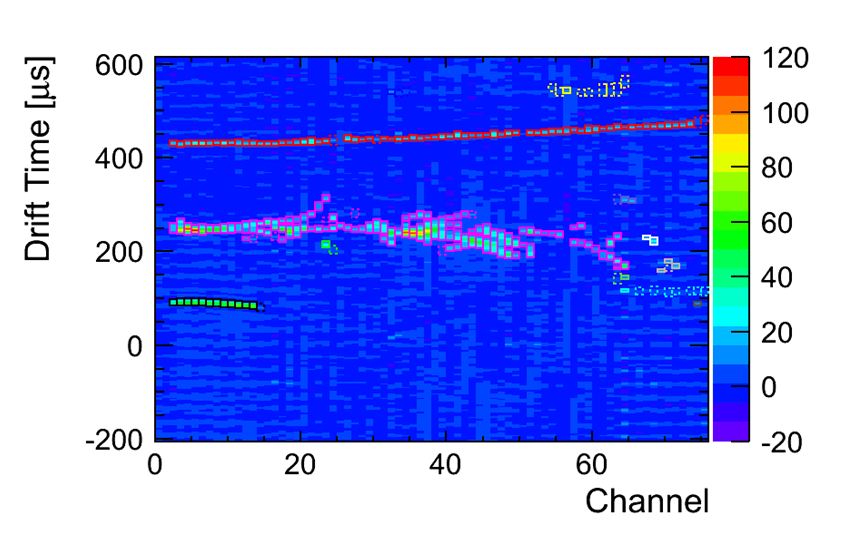
\includegraphics[width=60mm]{fig/clustering.eps}
 \end{center}
 \caption{Example of hit finding and clustering. A colored box corresponds to a hit and colors represent different clusters.}
 \label{fig:Clustering}
\end{figure}

\begin{itemize}
\item Plot: Finding efficiency vs threshold (Naganoma): TBU
\item Plot: Through-going pion data Q vs pion (Tanaka)
\end{itemize}
